\documentclass[11pt,a4paper]{article}
\usepackage[utf8]{inputenc}
\usepackage[T1]{fontenc}
\usepackage[norsk]{babel}
\usepackage{lmodern}
\usepackage[margin=2.5cm]{geometry}
\usepackage{amsmath}
\usepackage{graphicx}
\usepackage{booktabs}
\usepackage{xcolor}
\usepackage{enumitem}
\usepackage{float}
\usepackage[hidelinks]{hyperref}

\setlist{itemsep=1pt, topsep=3pt}
\setlength{\emergencystretch}{2em}
\newcommand{\todo}[1]{\textcolor{red}{[TODO: #1]}}
\newcommand{\code}[1]{\texttt{#1}}

\title{ML assignment 2 -- Phishing-lenkesjekk\\[4pt]\large DAT158, Høgskulen på Vestlandet}
\author{Jørn Kvittem \and Torgeir Hellebust}
\date{\today}

\begin{document}
\maketitle

\noindent\textbf{Live-app:} \url{https://huggingface.co/spaces/h189129/dat158-phishing-lenkesjekk}\\
\textbf{Kode:} \url{https://github.com/h189129/dat158-ml-assignment-2}

\noindent README-en i repoet beskriver alle detaljer og hvordan resultatene kan reproduseres.

% =====================================================================
\section{Beskriv problemet}

\paragraph{Mål.} Vi har laget en nettside der brukeren limer inn en lenke, for eksempel fra en mistenkelig e-post eller SMS, og får en vurdering av om lenken sannsynligvis fører til en phishing-side. Resultatet vises som et risikonivå (\emph{Lav risiko}, \emph{Mistenkelig} eller \emph{Høy risiko}) og en score fra 0 til 100. Vurderingen er et hjelpemiddel, ikke en garanti for at en lenke er trygg.

\paragraph{Hvorfor maskinlæring.} Svartelister er raske for kjente nettsteder, men kan ikke oppdage nye angrep som ikke er registrert ennå \cite{phreshphish}. En maskinlæringsmodell kan lære mønstre i hvordan phishing-adresser er bygget opp, for eksempel mange underdomener, merkenavn på uvanlige steder eller IP-adresser som vertsnavn. En enkel regelbasert løsning med slike regler fanget bare 23\,\% av phishing-lenkene i valideringsdataene.

\paragraph{Avgrensning.} Datasettet PhreshPhish \cite{phreshphish,datasetcard} inneholder URL og HTML. Vi bruker bare URL-en, og appen besøker aldri nettsiden. Det sparer ressurser og unngår kontakt med skadelige sider, men betyr at modellen ikke ser sideinnhold eller videresendinger. Lenkeforkortere (som bit.ly) skjuler målet og vurderes ikke. Produktet er en lenkesjekk, ikke et e-postfilter.

\paragraph{Metrikker.} Feiltypene har ulike konsekvenser. En phishing-lenke som slipper gjennom, kan føre til at brukeren oppgir passord eller kortinformasjon. Mange falske alarmer gjør at brukeren slutter å stole på verktøyet. Vi styrer derfor tersklene etter andelen falske alarmer blant legitime lenker (FPR) og maksimerer andelen phishing som fanges (recall) innenfor den grensen. Hovedmetrikken for modellvalg er \emph{recall ved 1\,\% FPR}. I tillegg rapporterer vi presisjon, F1, ROC-AUC og average precision (AP).

Presisjon avhenger av hvor stor andel av lenkene som er phishing. Testsettet har 44\,\% phishing, men i virkeligheten er andelen langt lavere. Vi rapporterer derfor også presisjon på datasettets benchmark-delmengder med 5\,\% og 1\,\% phishing.

Software-metrikken er responstid: minst 95\,\% av forespørslene skal besvares innen ett sekund.

\paragraph{Suksesskriterier.} Det opprinnelige målet var 90\,\% presisjon ved 90\,\% recall (P@R0,9), som i PhreshPhish-artikkelen \cite{phreshphish}. På valideringsdataene krevde 90\,\% recall at 52\,\% av de legitime lenkene ble flagget, så målet var ikke realistisk med URL alene. Det reviderte kriteriet var: høyest mulig recall ved 1\,\% FPR, klart bedre enn baselinene, og en FPR på testdata nær 1\,\%.

% =====================================================================
\section{Data}

PhreshPhish \cite{datasetcard} (CC BY 4.0) har 666\,315 nettsider fra juli 2024 til desember 2025. Vi låste datasettversjonen og leste bare kolonnene for URL, etikett, dato og etterlignet merkevare.

\paragraph{Funn i datautforskningen.} Datasettet hadde artefakter som ville gitt en modell med gode tall, men som ikke virker på ekte lenker:
\begin{itemize}
  \item \textbf{Query-strenger} (\code{?...}) fantes bare i phishing-URL-er. Modellen kunne lært at «\code{?} betyr phishing».
  \item \textbf{Skrivemåte:} i en tidlig prototype fikk \nolinkurl{https://www.nrk.no} score 0,99, mens samme adresse med skråstrek på slutten fikk 0,02.
  \item \textbf{Forsider:} bare 7\,\% av de legitime URL-ene var forsider, mot 47\,\% av phishing-URL-ene.
  \item \textbf{Innsamlingstidspunkt:} ingen legitime URL-er fra november 2024 til mai 2025.
  \item \textbf{Delte plattformer} (gitbook.io, webflow.io, docs.google.com o.l.) hadde nesten bare phishing.
\end{itemize}

\paragraph{Forbehandling.}
\begin{itemize}
  \item \textbf{Kanonisering:} alle URL-er normaliseres slik nettlesere tolker dem (WHATWG URL-standarden \cite{whatwg}). Skjema, \code{www.}, skråstrek på slutten, query-streng og fragment fjernes, både i trening og i appen.
  \item \textbf{Duplikater, konflikter og lenkeforkortere} fjernes.
  \item \textbf{Tidsbasert splitt} (tabell \ref{tab:splitt}): modellen evalueres alltid på data fra senere enn den er trent på, slik det er i drift.
  \item \textbf{Gruppering på nettsted} ved kryssvalidering (\code{GroupKFold}), slik at modellen må vurdere nye nettsteder i stedet for å huske kjente.
  \item \textbf{Datautvidelse:} er \code{nettsted/a/b} legitim, er også \code{nettsted/a} og \code{nettsted} det. Det ga 235\,710 ekstra legitime treningsrader og halverte falske alarmer på ekte legitime forsider (fra 8,9\,\% til 4,7\,\% på validering).
\end{itemize}

\begin{table}[H]
\centering
\small
\caption{Datasplitt etter rensing.}\label{tab:splitt}
\begin{tabular}{llrr}
\toprule
Sett & Periode & Legitime & Phishing \\
\midrule
Trening & jul.\ 2024 -- jun.\ 2025 & 181\,721 & 181\,550 \\
Validering (modellvalg og terskler) & jul.\ -- sep.\ 2025 & 94\,901 & 29\,274 \\
Test (én endelig evaluering) & sep.\ -- des.\ 2025 & 91\,199 & 72\,295 \\
\bottomrule
\end{tabular}
\end{table}

\paragraph{Kjennetegn (features).} Hver URL gjøres om til 69 tall: lengder, antall tegn som punktum, bindestreker og sifre, entropi, tekniske triks (IP-adresse, \code{@}, punycode), nøkkelord som «login» og «verify», merkenavn i domene, underdomene eller sti, delt plattform og toppdomene. To kjennetegn som oppførte seg ulikt fra måned til måned, ble fjernet fordi de sa mer om innsamlingstidspunktet enn om phishing.

% =====================================================================
\section{Modellering}

Vi sammenlignet to baselines og fire modeller fra pensum \cite{geron}. Alle er bygget som en scikit-learn-\code{Pipeline} \cite{sklearn} der første steg beregner kjennetegnene, slik at appen bruker samme kode som treningen. Hyperparametre ble valgt med \code{RandomizedSearchCV} og 3-fold \code{GroupKFold}.

Utvalgsregelen ble bestemt på forhånd: høyest recall ved 1\,\% FPR på validering, for modeller under 50\,MB og 100\,ms per URL.

\begin{table}[H]
\centering
\small
\caption{Modellvalg på valideringsdata (24\,\% phishing).}\label{tab:modellvalg}
\begin{tabular}{lrrrr}
\toprule
Modell & ROC-AUC & Recall ved 1\,\% FPR & Størrelse & Tid per URL \\
\midrule
Dummy (andel phishing) & 0,500 & 0 & -- & -- \\
Regelbasert baseline & 0,603 & --\textsuperscript{a} & -- & -- \\
Logistisk regresjon & 0,849 & 0,455 & $<$0,1\,MB & 0,5\,ms \\
Beslutningstre & 0,867 & 0,568 & 0,1\,MB & 0,3\,ms \\
Random forest & 0,907 & 0,591 & 8,6\,MB & 25\,ms \\
\textbf{Gradient boosting (valgt)} & 0,888 & \textbf{0,617} & 0,5\,MB & 3\,ms \\
\bottomrule
\end{tabular}\\[2pt]
\footnotesize\textsuperscript{a} Reglene gir recall 22,6\,\% ved FPR 1,9\,\%.
\end{table}

Random forest har høyest ROC-AUC, men gradient boosting har høyest recall når falske alarmer holdes lave, og det er det som betyr noe for brukeren. Den er også 17 ganger mindre og 8 ganger raskere.

Kryssvalideringen ga ROC-AUC 0,99, men valideringsdataene fra senere måneder bare 0,89. Phishing endrer seg over tid, og kryssvalidering innenfor samme periode gir et for optimistisk bilde. Derfor brukte vi den tidsbaserte valideringen til modellvalg og terskler.

\paragraph{Terskler.} Satt på validering: \emph{Høy risiko} fra score 55 (FPR 1\,\%) og \emph{Mistenkelig} fra score 13 (FPR 5\,\%).

\paragraph{Feilanalyse.} På validering ga legitime sider på delte plattformer 25\,\% falske alarmer, og phishing på kompromitterte, ekte nettsteder (f.eks.\ \code{.gov}) ble nesten aldri fanget. De viktigste kjennetegnene (permutation importance) var lengden på vertsnavnet, antall ord i adressen, delt plattform, nøkkelord og https. Læringskurven steg fortsatt med all treningsdata, så mer data vil sannsynligvis hjelpe.

\paragraph{Testresultater.} Modellen og tersklene ble låst før testsettet ble kjørt.

\begin{table}[H]
\centering
\small
\caption{Testresultater (162\,531 URL-er, 44\,\% phishing).}\label{tab:test}
\begin{tabular}{lrrr}
\toprule
 & Høy risiko & Mistenkelig & Lav risiko \\
\midrule
Faktisk phishing & 69,7\,\% & 16,5\,\% & 13,9\,\% \\
Faktisk legitim & 1,2\,\% & 4,3\,\% & 94,6\,\% \\
\bottomrule
\end{tabular}

\vspace{6pt}
\begin{tabular}{lr}
\toprule
ROC-AUC / AP & 0,960 / 0,961 \\
\emph{Høy risiko}: presisjon / recall / FPR / F1 & 97,9\,\% / 69,7\,\% / 1,2\,\% / 0,81 \\
Presisjon ved 5\,\% og 1\,\% phishing (benchmark) & 75,9\,\% og 37,7\,\% \\
P@R0,9 på hele testsettet / ved 5\,\% / ved 1\,\% phishing & 88,6\,\% / 21,6\,\% / 5,1\,\% \\
\bottomrule
\end{tabular}
\end{table}

86\,\% av phishing-lenkene får en advarsel, men 13,9\,\% slipper gjennom som \emph{Lav risiko}. FPR på test (1,2\,\%) ble nær målet. Ved 1\,\% phishing er bare 38\,\% av varslene om \emph{Høy risiko} ekte, slik Bayes' regel forutsier ut fra recall og FPR.

Til sammenligning oppnår den svakeste modellen i PhreshPhish-artikkelen, som bruker både URL og HTML, AP 0,684 ved 1\,\% phishing \cite{phreshphish}. Vår URL-modell får 0,622. Sammenligningen er ikke eksakt, fordi vi bare evaluerer de benchmark-radene som er igjen etter vår rensing.

\paragraph{Åpenhet om metode.} Testsettet er kjørt to ganger. Etter første kjøring (modell v1) avdekket en manuell sjekk på norske nettsteder en kodefeil: merkenavn ble funnet inni andre ord («posten» i «aftenposten»). Vi rettet feilen og flere andre, trente og valgte modellen på nytt med bare trenings- og valideringsdata, og kjørte testen én gang til (v2, tallene over). Testtallene fra v1 ble ikke brukt til beslutninger, men var kjent.

% =====================================================================
\section{Deployment}

Appen er laget med Gradio \cite{gradio} og publisert på Hugging Face Spaces. Hugging Face krever fra sommeren 2026 et PRO-abonnement for Gradio-apper \cite{hfspaces}, så appen kjører på en PRO-konto.

\begin{itemize}
  \item \textbf{Samme kode i trening og drift:} modellen er lagret som én \code{Pipeline} (0,47\,MB). En sjekksum av koden for kjennetegn hindrer at appen starter hvis koden er endret etter treningen.
  \item \textbf{Grensesnitt} (figur \ref{fig:app}): risikonivå, score på en skala med tersklene markert, en anbefaling, og adressen med domenet som eier den uthevet. Uthevingen viser brukeren hvem som faktisk eier en adresse som \code{secure-dnb-login.verify-account.xyz}. Appen fungerer på mobil og PC.
  \item \textbf{Responstid:} 95\,\% av forespørslene besvares innen 106\,ms lokalt fra klikk til resultat. Selve vurderingen tar under 5\,ms.
  \item \textbf{Overvåking:} vi spilte av testmånedene som ny trafikk med en regel for ny trening (FPR over 2 ganger valideringsnivået, eller recall mer enn 0,10 under). Regelen slo til i september 2025, da recall falt til 36\,\% på grunn av phishing på kompromitterte nettsteder.
  \item \textbf{Personvern:} appen åpner aldri lenken og lagrer ikke det brukeren limer inn.
\end{itemize}

\begin{figure}[H]
\centering
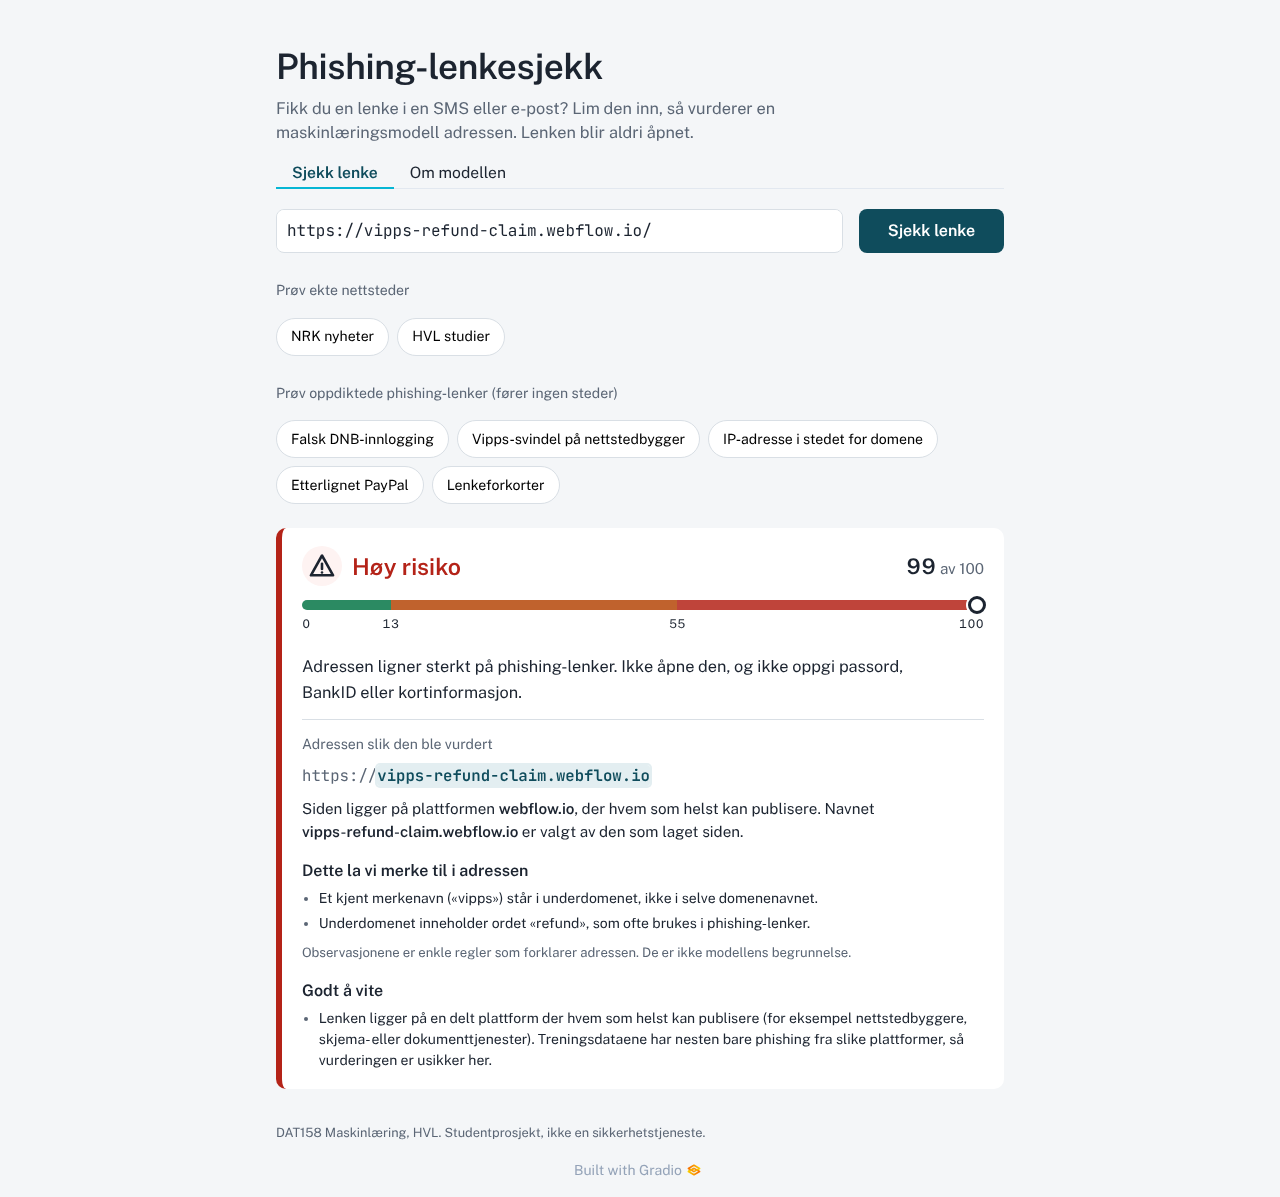
\includegraphics[height=7.5cm]{figurer/app_sjekk_lenke.png}\hfill
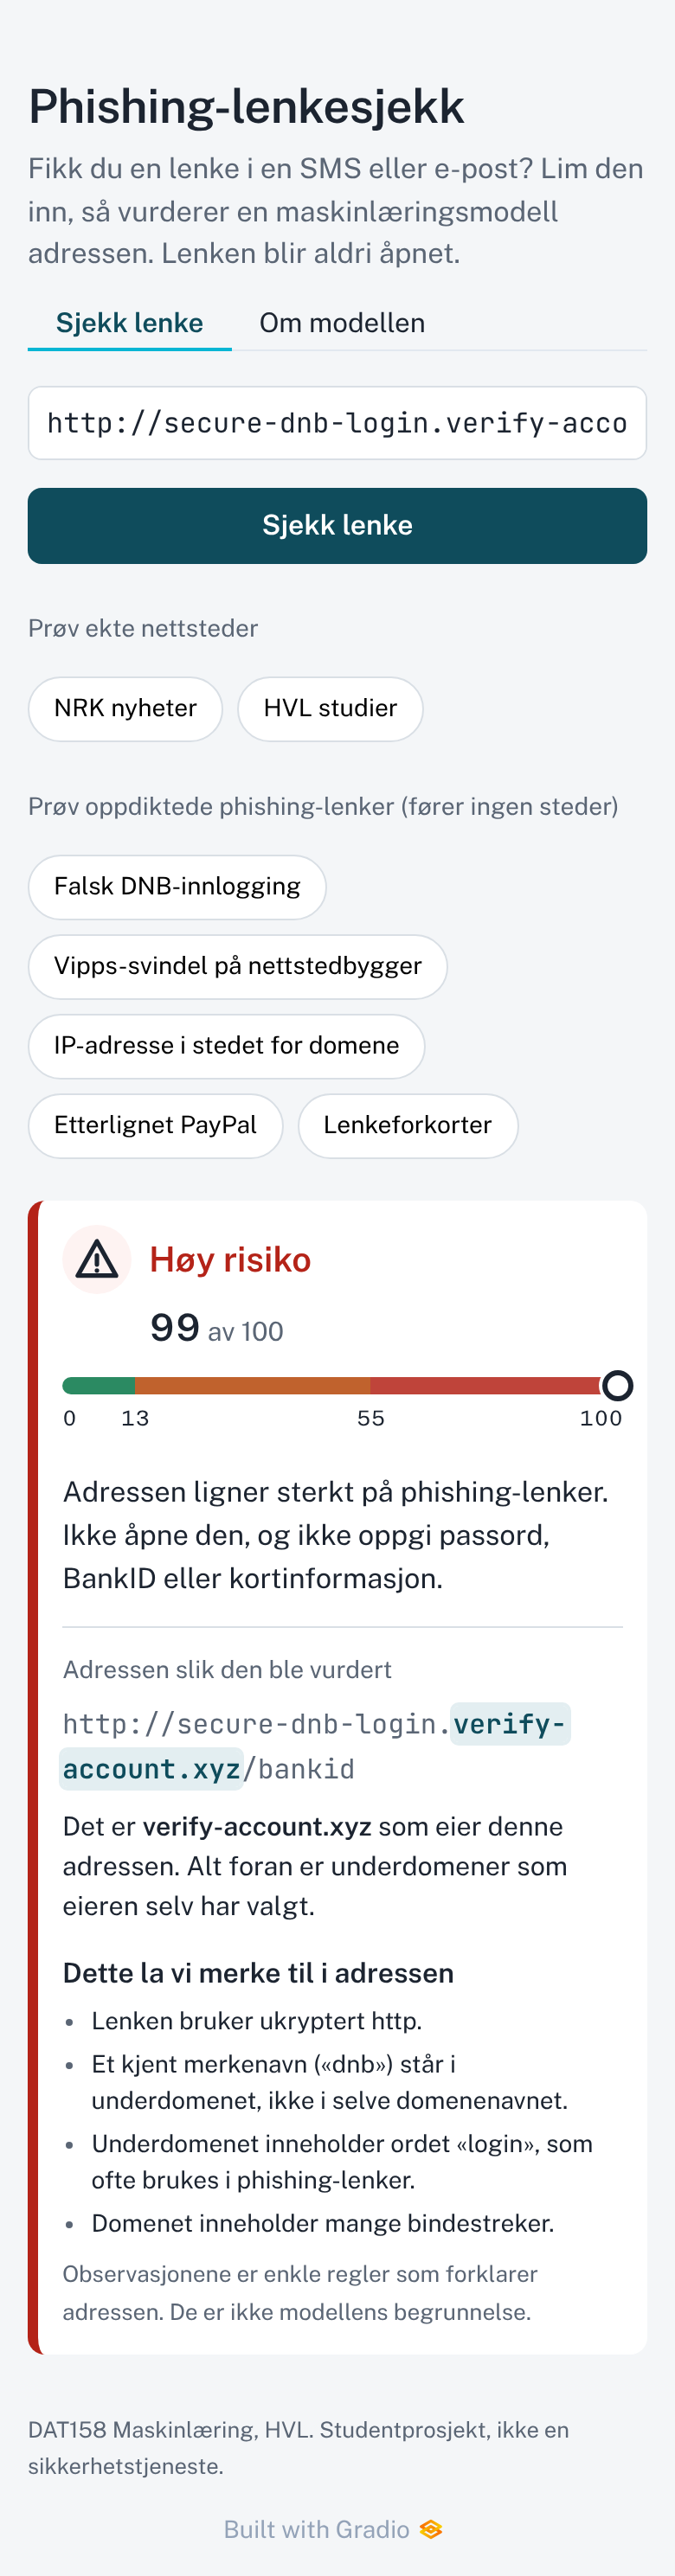
\includegraphics[height=7.5cm]{figurer/app_mobil.png}
\caption{Appen på PC og mobil.}\label{fig:app}
\end{figure}

% =====================================================================
\section{Diskusjon og konklusjon}

Modellen fanger 70\,\% av phishing-lenkene som \emph{Høy risiko} og 86\,\% med en eller annen advarsel, med 1,2\,\% falske alarmer på data fra senere måneder enn treningen. Det viktigste vi lærte, er at datasettets artefakter ville gitt imponerende, men misvisende tall. Kanonisering, datautvidelse, tidsbasert splitt og gruppering på nettsted gir lavere, men mer ærlige resultater.

\paragraph{Begrensninger.} Phishing på kompromitterte, ekte nettsteder er usynlig i adressen. Ved realistisk andel phishing er presisjonen lav. Norske nettsteder er sjeldne i dataene, og korte domenenavn med tall (\code{tv2.no}) får for høy score. Legitime sider på delte plattformer og sider uten https vurderes for strengt.

\paragraph{Videre arbeid.} Tegn-n-grammer fra URL-en, sideinnholdet (HTML) eller oppslag som domenets alder ville trolig gitt bedre resultater. De to siste bryter med avgrensningen vår.

Modellen er derfor best egnet som et raskt og personvernvennlig førstefilter, i kombinasjon med andre signaler, og ikke som eneste beskyttelse.

\section*{Bruk av KI-verktøy}
Vi brukte Claude (Anthropic) som verktøy gjennom hele prosjektet: til sparring om problemstilling og metode, til analyse av datasettet, der den blant annet hjalp oss å avdekke artefaktene beskrevet i avsnitt 2, og til å generere koden for pipeline, modeller, evaluering, app og tester. Den ga også et utkast til struktur og tekst for rapporten, som vi har bearbeidet. Vi valgte problem, datasett og avgrensning (bare URL), godkjente prosjektplanen og avgjorde de viktigste valgene underveis: hvordan tersklene skulle styres, og at en feil oppdaget etter første testkjøring skulle rettes med en ny, dokumentert modellversjon. Vi har testet og publisert appen, og står ansvarlige for innholdet.

% =====================================================================
\begin{thebibliography}{9}
\small
\bibitem{phreshphish}
T.~Dalton, H.~Gowda, G.~Rao, S.~Pargi, A.~H.~Khodabakhshi, J.~Rombs, S.~Jou, and M.~Marwah.
\newblock PhreshPhish: A real-world, high-quality, large-scale phishing website dataset and benchmark.
\newblock \emph{arXiv preprint arXiv:2507.10854}, 2025.

\bibitem{datasetcard}
PhreshPhish dataset card. Hugging Face, \url{https://huggingface.co/datasets/phreshphish/phreshphish}. Lest 2026-10-26.

\bibitem{geron}
A.~Géron. \emph{Hands-On Machine Learning with Scikit-Learn, Keras \& TensorFlow}, 3.~utg. O'Reilly, 2022.

\bibitem{sklearn}
F.~Pedregosa mfl. Scikit-learn: Machine learning in Python. \emph{JMLR}, 12:2825--2830, 2011. Versjon 1.9.1.

\bibitem{whatwg}
WHATWG. URL Living Standard. \url{https://url.spec.whatwg.org/}. Lest 2026-10-26.

\bibitem{gradio}
Gradio, versjon 6.30.0. \url{https://www.gradio.app/}.

\bibitem{hfspaces}
Hugging Face. Spaces Overview. \url{https://huggingface.co/docs/hub/en/spaces-overview}. Lest 2026-10-26.
\end{thebibliography}

\end{document}
